\subsection{Introduction}
The task for group 1 in phase 1 was to specify energy relevant attributes and try to calculate or extract them from the semantic city model.\\
First of all a connection to the database was necessary to establish, and the following three subtasks where reasonable to define.
With the specification of the energy relevant attributes inside of the database, a data basis for the different algorithms was created. This algorithms can be differentiated into data analysis algorithms basing on the pure values stored in the database and geometry analysis dealing with the geometry information in the database.\\
Our work was restricted to the area of Berlin Moabit, a small subset of the full Berlin model. For the Java algorithms the database information where exported as .gml files and the obtained output was saved as .csv files, which were able to be re-uploaded to the database. All data kept their necessary identifier.\\
As important values for an energy atlas following parameter where determined:
\begin{itemize}
\item Airvolume of building to be able to calculate the Surface-to-Volume-Ratio
\item Number of storeys which can be calculated by using the average storey-height of the specific building
\item Orientation of the wallsurfaces of each building to get information about neighbourhood relations between buildings and inner- and outer walls
\end{itemize}

\subsection{Data Analysis}
Each building stored in the database contains at least one groundsurface, one roofsurface and three wallsurfaces. Based on these information, the volume of the buildings, the orientation of the walls (whether it is a outer or neighbouring wall), therewith also the surface-to-volume-ratio and the outer-wall orientation for sunlight-heating-effects can be calculated. Also necessary for the average storey height and important for the calculations is the building’s function as it is residential, public or industry.\\
Moreover, we identified some missing energy relevant data like the building's year of construction. With this it is possible to estimate the building's material, the mean size of windows, the type of windows, and the mean story height. In addition, the topological relations between buildings are missing, as well as the number of people living in the building resp. number of flats, and the behaviour classes of the people living in the building (to estimate their energy consumption).

\subsection{Geometry Analysis}
In the geometry analysis we mainly focused on the surface area to volume ratio as well as the outer orientation of the walls. Carrion \citep{carrion2010} defines the surface area to volume ratio as follows:
\begin{quote}
"The S/V is the ratio of the aggregated area of all surfaces which transmit energy to the surrounding (wall surfaces touching other buildings are not considered) and the volume of the building."
\end{quote}
To calculate the S/V ratio, we created two subtasks. One task is to calculate for each building the area which is touching neighbouring buildings as well as to calculate the sum of all surface areas of one building. The second task is to calculate the volume of each building.

\subsection{Calculation of wall-surface intersection}
Important to know is, that the S/V does not include wall surfaces touching other buildings, and therewith those wallsurfaces must be detected using the information which are stored in the database. For this issue the following workflow to calculate wall surfaces which are not touching other buildings was developed:
\begin{enumerate}
\item Calculate neighbouring buildings
\item Calculate area touching other buildings (for each building)
\item Calculate sum of surface areas (ground-, roof-, wallsurfaces)
\item Subtract intersecting area with neighbouring building from sum of surface areas
\end{enumerate}

\subsubsection{Calculate neighbouring buildings}
The calculation of neighbouring buildings is done, to minimize the candidate set for the calculation of the intersection of two buildings. Two buildings are neighboured if the wall surfaces of the two buildings are within a certain distance, and the angle between wall surfaces is smaller than a defined threshold (see figure \ref{fig:neighbours3d}). 
Since we did the calculation in Java with the JTS Topology Suite (JTS), the problem was that JTS is not able to do calculations on 3D geometries. A workaround is to make the assumption, that the wall surfaces are vertical and parallel to each other. Then a projection of the walls into 2D can be done by ignoring the Z coordinates.
\begin{figure}[h]
	\centering
 	 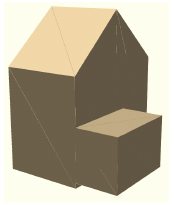
\includegraphics[scale=0.35]{phase1/group1/neighbours3d.png}
	\caption{Neighboured buildings in 3D.}
	 \label{fig:neighbours3d}
\end{figure}
This means, every wall surface becomes a linestring (see figure \ref{fig:neighbours2d}).
\begin{figure}[h]
	\centering
 	 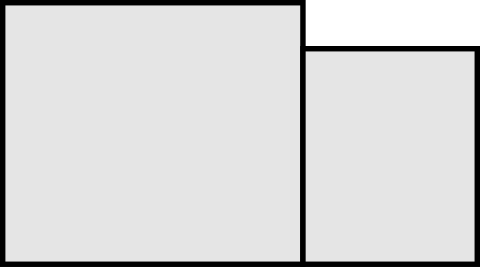
\includegraphics[scale=0.8]{phase1/group1/neighbours2d.png}
	\caption{Neighboured buildings in 2D.}
	\label{fig:neighbours2d}
\end{figure}
Then we can test if two walls represented by linestrings are within a certain distance and the angle between the linestrings is smaller than a threshold using JTS.

\subsubsection{Calculating area touching other buildings}
After determining if two buildings are neighboured, it is possible to calculate the intersection area of touching wall surfaces. Since JTS is not able to do calculations on 3D geometries, as mentioned above, the walls need to be transformed to 2D again. Therefore the coordinate system has to be transformed so that the wall surfaces are lying in the YZ-plane. Then, the X coordinate can be ignored and the intersection of the two walls can be calculated.\\
To rotate the coordinate system so that the wall surfaces are lying in the YZ-plane, the normal vector of one of the two walls has to be calculated. With this the rotation angle $\alpha$ can be calculated as the angle between the normal vector on the vector [1 0 0], which is the normal of the YZ-plane. Then both wall surfaces are rotated with this rotation angle $\alpha$. Figure \ref{fig:rotation_matrix} shows the used rotation matrix.
\begin{figure}[h]
	\centering
 	 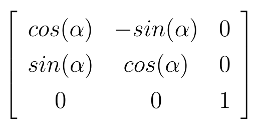
\includegraphics[scale=0.5]{phase1/group1/rotation_matrix.png}
	\caption{Rotation matrix used for calculating intersection.}
	\label{fig:rotation_matrix}
\end{figure}
If these rotated surfaces are intersecting, the real world surfaces are intersecting, too. Thus, the intersection of the rotated surfaces can be calculated as in the following listing:\\
\begin{lstlisting}[language=Java]
Geometry intersection=polygon.intersection(polygonNeighbour);
if (intersection instanceof com.vividsolutions.jts.geom.Polygon) {
  com.vividsolutions.jts.geom.Polygon intersectionPolygon 
  = (com.vividsolutions.jts.geom.Polygon) intersection;
  // unit is m^2
  intersectingArea = intersectionPolygon.getArea();
}
\end{lstlisting}

\subsubsection{Overall- and sharing wall area}
This is followed by the area calculation of the wall-, roof- and groundsurfaces for each building. These surface areas are summed up to get the overall surface area of each building.
These results (the surface areas of each building (building id)) are written to a .csv file to be able to import it back into the 3D city model database. Table \ref{table:result shared wall surfaces} shows some sample results.
\begin{table}[b]
\centering
\begin{tabular}{c  c  c}
building\_id & surface\_area & shared\_wall\_area\\
\hline						
BLDG\_0003000000432cd8 & 234.99638499102912 & 45.46462674214126\\
BLDG\_0003000000432c80 & 1265.0716547126067 & 529.4226535306225\\
BLDG\_0003000f000858d0 & 2201.2130139165056 & 975.798086083496\\
...\\
\end{tabular}
\caption{Subset of result .csv file containing shared wall surfaces.} 
\label{table:result shared wall surfaces}
\end{table}

\subsection{Geometry Analysis - Building Volume}
The building's volume can be calculated using several different approaches. The task is to have a volume which is a good approximation of the real existing air volume inside of the building, because it will be used afterwards for some energy-flow calculations. Necessary also for an operatively used approach is the automatisation of the algorithm and the potential for for its embedding into the other code.\\
The following approaches have been tested and checked whether they fulfil the requirements:
\begin{enumerate}
\item SQL algorithm/query
\item FME Software
\item ArcMap Software - 3D Analyst
\item ArcMap Software - Buildings to DEM
\end{enumerate}


\subsubsection{Volume calculation 1. approach: SQL}
Using SQL (Structured Query Language) as a possibility to directly access the database and analyse the stored information is the first upcoming option. For the calculation several Oracle spatial functions have been used to get the building area. Multiplying this with the building's height which is already stored in the database leads to a good estimation of the building's volume.\\
But the differences between the building's roof structure leads to wrong estimations of a large percentage of the building's volume, because only one height can be taken from the database which is the distance between the ground up to the highest roof point. The figure \ref{fig:build_h} is showing a good example of a possible wrong estimation: The different building parts are stored using only one building identifier, and therewith only the height of the highest part is stored inside of the database.
\begin{figure}[h]
	\centering
 	 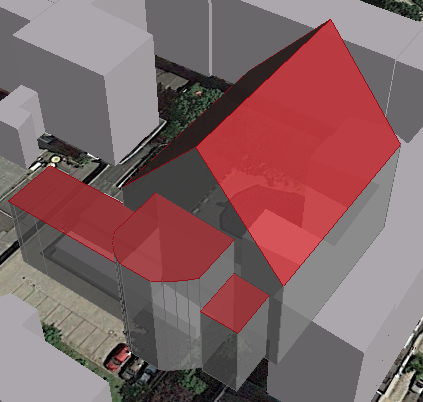
\includegraphics[scale=0.3]{phase1/group1/build_h.png} 
	\caption{Example of a more complex roof sturcture.}
	\label{fig:build_h}
\end{figure}

\subsubsection{Volume calculation 2. approach: FME}
The second approach was using the software FME (Feature Manipulating Engine). It’s FME Data Inspector shows the stored geometry and the buildings do not contain ground-, wall- and roofsurfaces (see figure \ref{fig:fme}). But the surfaces were represented as not connected so a building is not containing one closed geometry.\\
Since the FME workbench is very complex also a lot of errors occur, and therewith this approach is not really stable.
\begin{figure}[h]
	\centering
 	 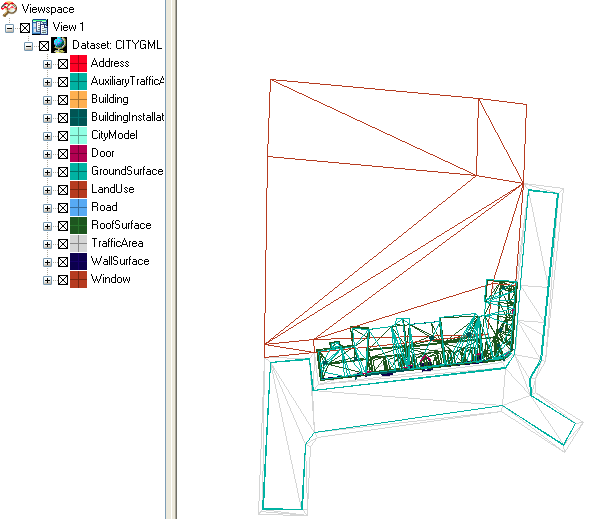
\includegraphics[scale=0.3]{phase1/group1/fme.png} 
	\caption{Visualisation of FME Data Inspector.}
	\label{fig:fme}
\end{figure}

\subsubsection{Volume calculation 3. approach: Arcmap}
The Software Arc Map offers an extension called 3D Analysed which can be used as an analysis tool for 3D objects.\\
In here it was possible to enclose the geometries of the buildings, but this procedure uses a shrinking of the building until every surface is completely touching its neighbours. Therewith the obtained volume of the building in systematically falsificated.

\subsubsection{Volume calculation 4. approach: Arcmap again}
For the last approach another functionality of Arc Map can be used: The creation of a rasterlayer for ground- and roof- geometries with the extension: "Add Buildings to DEM".\\
A complex sequence of operations have to be applied to first create a difference raster which is showing ground level and roof level and secondly calculating the volume using this raster.\\
For the automatisation the Arc Map Modelbuilder can be used. With this every step can be defined as an output and input of others. Figure \ref{fig:arcmap_raster} is showing the process.
\begin{figure}[h]
	\centering
 	 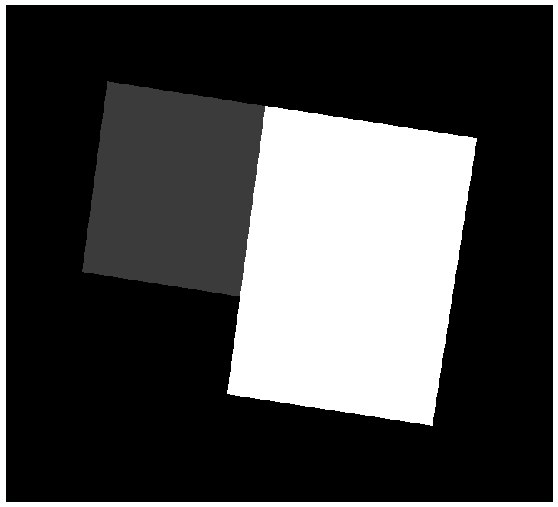
\includegraphics[scale=0.1]{phase1/group1/raster_ground.jpg} 
	 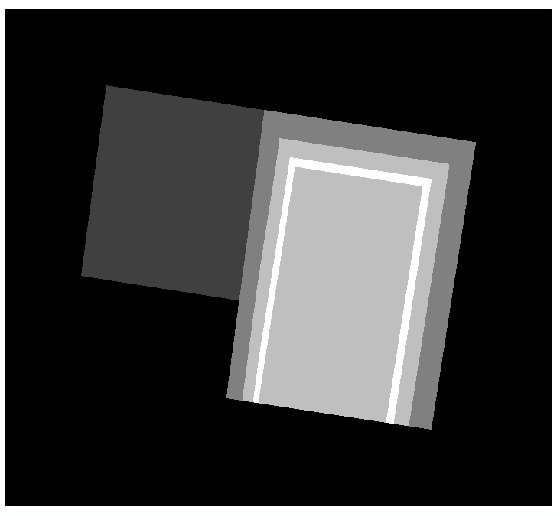
\includegraphics[scale=0.1]{phase1/group1/raster_roof.jpg}
	 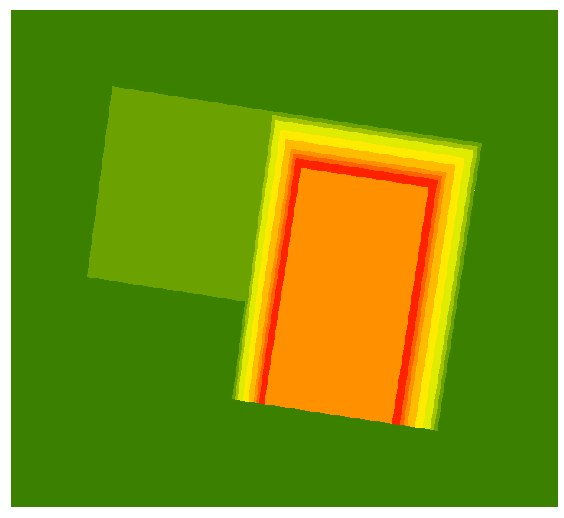
\includegraphics[scale=0.1]{phase1/group1/raster_diff.jpg} 
	 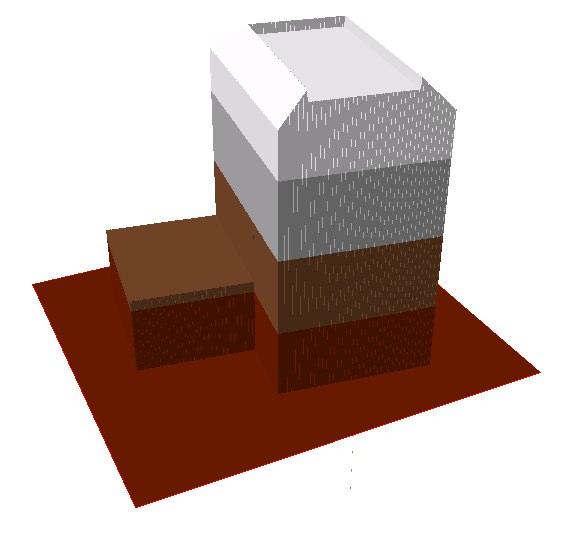
\includegraphics[scale=0.1]{phase1/group1/arcscene_tin.jpg} 
	 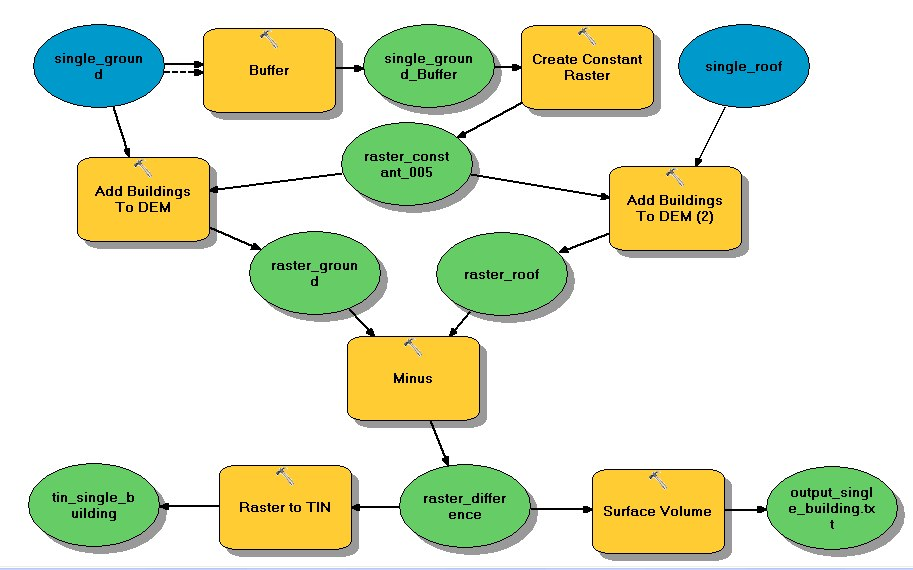
\includegraphics[scale=0.1]{phase1/group1/modelbuilder.jpg} 
	\caption{Visualisation of the 4th approach to calculate the volume.}
	\label{fig:arcmap_raster}
\end{figure}

\subsubsection{Volume calculation - Comparison}
Since our knowledge about the buildings is only depending on our data, a valid number of volume cannot be calculated without any statistical analysis of the buildings and the different calculations.\\
The table \ref{table:comparison_volume} shows a comparison of the different obtained results which.
\begin{table}[b]
\centering
\begin{tabular}{c  c  c}
Approach & calculated volume\\
\hline						
SQL & $10227m^3$\\
FME & no result\\
3D Analyst & $6000m^3$\\
Arc Map & $7400m^3$\\
\end{tabular}
\caption{Comparison of the different volume calculation procedures.} 
\label{table:comparison_volume}
\end{table}
